
\begin{figure}[h]
    \centering
    \begin{subfigure}[b]{0.32\linewidth}
        \centering
        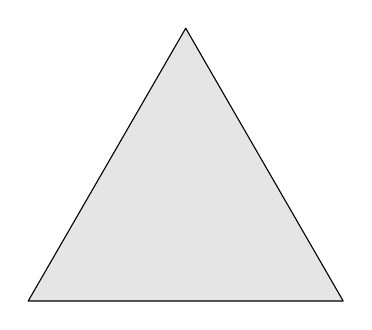
\begin{tikzpicture}[line cap=round,line join=round,x=1cm,y=1cm, scale=4]
          \coordinate (A) at (0,0);
          \coordinate (B) at (1,0);
          \coordinate (C) at (0.5,0.866);
    
          \fill[fill=black,fill opacity=0.1] (A) -- (B) -- (C) -- cycle;
    
          \draw (A) -- (B) -- (C) -- cycle;
  
        \end{tikzpicture}
        \caption{$F_0$.}
    \end{subfigure}
    \begin{subfigure}[b]{0.32\linewidth}
      \centering
      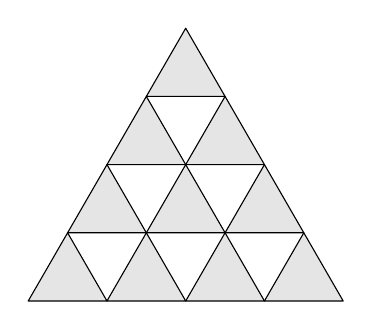
\begin{tikzpicture}[line cap=round,line join=round,x=1cm,y=1cm, scale=1]
  
        \foreach \i in {0,...,3}{
          \pgfmathsetmacro{\a}{3 - \i}
          \foreach \j in {0,...,\a}{
            \coordinate (A) at (0 + \i + 0.5*\j, 0 + 0.866*\j);
            \coordinate (B) at (1 + \i + 0.5*\j, 0 + 0.866*\j);
            \coordinate (C) at (0.5 + \i + 0.5*\j, 0.866 + 0.866*\j);
  
            \fill[fill=black,fill opacity=0.1] (A) -- (B) -- (C) -- cycle;
            \draw (A) -- (B) -- (C) -- cycle;
          }
        }
      \end{tikzpicture}
      \caption{$F_1$.}
    \end{subfigure}
    \begin{subfigure}[b]{0.32\linewidth}
      \centering
      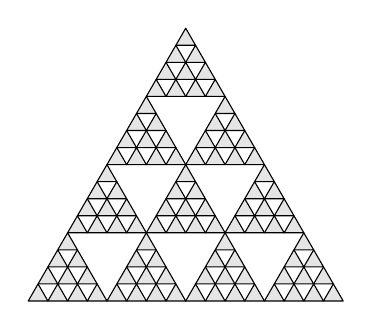
\begin{tikzpicture}[line cap=round,line join=round,x=1cm,y=1cm, scale=0.25]
      \foreach \k in {0,...,3}{
        \pgfmathsetmacro{\b}{3 - \k}
        \foreach \h in {0,...,\b}{
          \foreach \i in {0,...,3}{
            \pgfmathsetmacro{\a}{3 - \i}
            \foreach \j in {0,...,\a}{
              \coordinate (A) at (0 + \i + 0.5*\j + 4*\k + 2*\h,
                                  0 + 0.866*\j + 0.866*4*\h);
              \coordinate (B) at (1 + \i + 0.5*\j + 4*\k + 2*\h,
                                  0 + 0.866*\j + 0.866*4*\h);
              \coordinate (C) at (0.5 + \i + 0.5*\j + 4*\k + 2*\h,
                                  0.866 + 0.866*\j + 0.866*4*\h);
  
              \fill[fill=black,fill opacity=0.1] (A) -- (B) -- (C) -- cycle;
              \draw (A) -- (B) -- (C) -- cycle;
            }
          }
        }
      }
      \end{tikzpicture}
      \caption{$F_2$.}
    \end{subfigure}
    \caption{Primeras iteraciones del fractal semejante al triángulo de Sierpinski.}
    \label{fig:triangles}
  \end{figure}